% Code tour — how the repository folders work together.
% Companion to docs/guidebook (physics/statistics); this document is about
% the CODE. Mirrors the guidebook's palette, fonts, and box styles so the
% two PDFs read as one family. Source of truth for prose: docs/CODE_TOUR.md.
\documentclass[11pt]{article}

\usepackage[a4paper,margin=2.2cm]{geometry}
\usepackage[T1]{fontenc}
\usepackage{newtxtext,newtxmath}
\usepackage[scaled=0.90]{helvet}
\usepackage{microtype}
\usepackage{amsmath}
\usepackage{booktabs}
\usepackage{array}
\usepackage{tabularx}
\usepackage{xcolor}
\usepackage[most]{tcolorbox}
\usepackage{enumitem}
\usepackage{titlesec}
\usepackage{fancyhdr}
\usepackage[hidelinks]{hyperref}
\usepackage{tikz}
\usetikzlibrary{positioning, arrows.meta, calc, fit, backgrounds, shapes.geometric}

% ---- house palette (matches docs/guidebook/guidebook.tex) ----
\definecolor{forest}{HTML}{3D6E4A}
\definecolor{coral}{HTML}{B85B3A}
\definecolor{teal}{HTML}{2C6E73}
\definecolor{char}{HTML}{2B2B2B}
\definecolor{dim}{HTML}{6B6B6B}
\definecolor{rulec}{HTML}{C9C2B6}
\definecolor{codebg}{HTML}{F4F2EE}

\color{char}
\newcommand{\code}[1]{{\ttfamily\small #1}}

% ---- section styling (matches the guidebook) ----
\titleformat{\section}{\normalfont\sffamily\Large\bfseries\color{forest}}{\thesection}{0.6em}{}
\titleformat{\subsection}{\normalfont\sffamily\large\bfseries\color{char}}{\thesubsection}{0.5em}{}
\titlespacing*{\section}{0pt}{14pt}{6pt}
\titlespacing*{\subsection}{0pt}{10pt}{4pt}

\pagestyle{fancy}
\fancyhf{}
\renewcommand{\headrulewidth}{0.3pt}
\fancyhead[L]{\small\sffamily\color{dim}Apollo $K_d$ --- code tour}
\fancyhead[R]{\small\sffamily\color{dim}\thepage}

% ---- callout boxes (same styles as the guidebook) ----
\newtcolorbox{rule box}[1][]{colback=forest!7,colframe=forest!55,boxrule=0.7pt,arc=2pt,
  left=6pt,right=6pt,top=3pt,bottom=3pt,before skip=6pt,after skip=6pt,
  title={\sffamily\bfseries The one rule},coltitle=forest,fonttitle=\small,#1}
\newtcolorbox{housebox}[1][]{colback=teal!5,colframe=teal!45,boxrule=0.6pt,arc=2pt,
  left=7pt,right=7pt,top=5pt,bottom=5pt,before skip=6pt,after skip=6pt,#1}

\title{\sffamily\bfseries\color{forest}\LARGE Code tour\\[2pt]
  \large\normalfont\color{char} How the repository folders work together}
\author{}
\date{\small\sffamily\color{dim}Companion to \code{docs/guidebook/} (physics \& statistics) --- this document is about the code}

\begin{document}
\maketitle
\thispagestyle{fancy}
\vspace{-1.2cm}

\tableofcontents
\vspace{0.4cm}

% =====================================================================
\section{The mental model: four layers, one rule}
% =====================================================================

The repository is four layers, each one built on the last. Data comes in at
the top; the engine turns data into physics; the pipeline turns physics into
numbers; the documents turn numbers into prose and figures. Two more folders
--- \code{notebooks/} and \code{tests/} --- sit beside this spine rather than
inside it: notebooks are an interactive front door onto the same layers,
tests are guardrails clamped onto the engine.

\begin{figure}[h]\centering
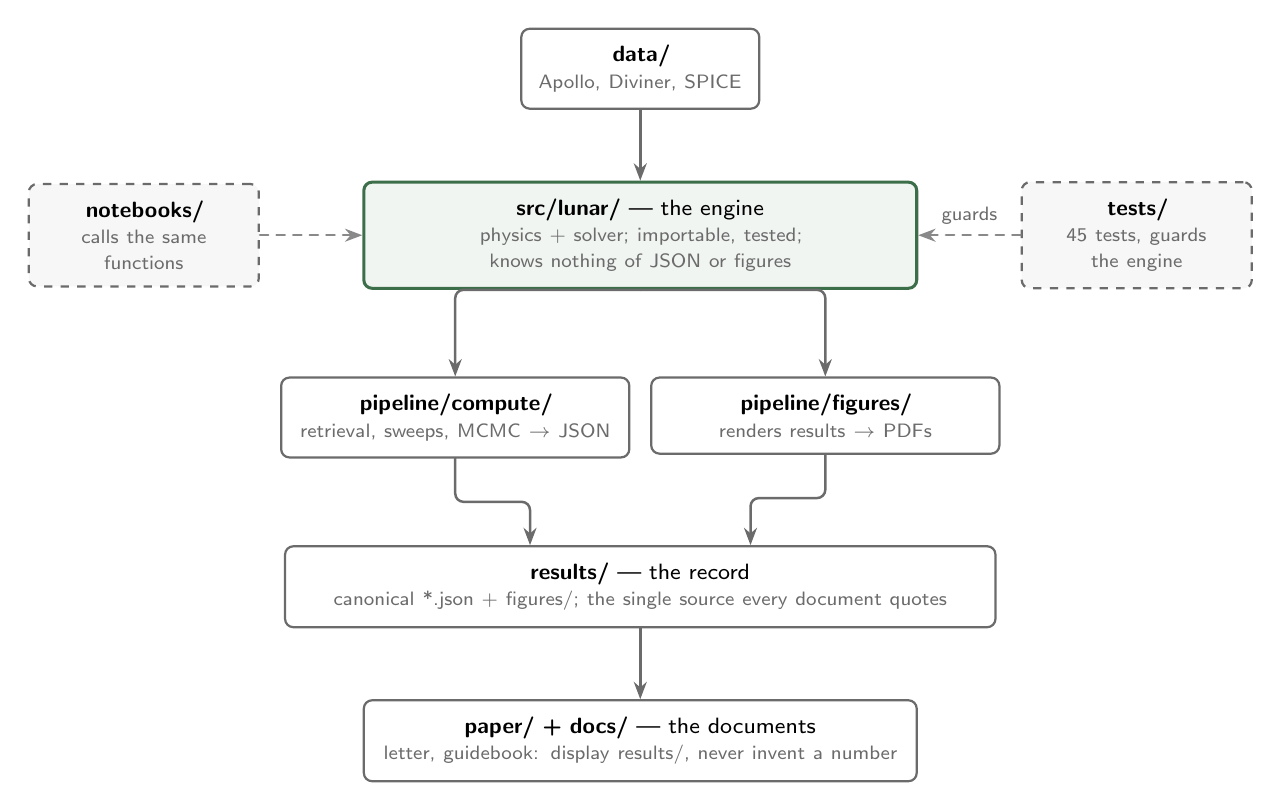
\begin{tikzpicture}[
  font=\sffamily\footnotesize,
  every node/.style={align=center},
  box/.style={rectangle, rounded corners=3pt, draw=dim, line width=0.8pt,
              fill=white, inner sep=6pt},
  engine/.style={box, draw=forest, line width=1.1pt, fill=forest!7},
  side/.style={box, draw=dim, dashed, fill=black!3, text width=2.5cm},
  arr/.style={-{Stealth[length=2.2mm]}, line width=0.9pt, draw=dim,
              rounded corners=3pt, line cap=round},
  darr/.style={arr, dashed, draw=dim!80}
]
  \node[box, text width=2.6cm] (data) at (0,0) {\textbf{data/}\\{\scriptsize\color{dim}Apollo, Diviner, SPICE}};
  \node[engine, below=9mm of data, text width=6.6cm] (engine)
    {\textbf{src/lunar/} --- the engine\\{\scriptsize\color{dim}physics + solver; importable, tested; knows nothing of JSON or figures}};
  \node[box, below=11mm of engine, xshift=-2.35cm, text width=4.0cm] (compute)
    {\textbf{pipeline/compute/}\\{\scriptsize\color{dim}retrieval, sweeps, MCMC $\rightarrow$ JSON}};
  \node[box, below=11mm of engine, xshift=2.35cm, text width=4.0cm] (figs)
    {\textbf{pipeline/figures/}\\{\scriptsize\color{dim}renders results $\rightarrow$ PDFs}};
  \node[box, below=11mm of compute, xshift=2.35cm, text width=8.6cm] (results)
    {\textbf{results/} --- the record\\{\scriptsize\color{dim}canonical *.json + figures/; the single source every document quotes}};
  \node[box, below=9mm of results, text width=6.6cm] (docs)
    {\textbf{paper/ + docs/} --- the documents\\{\scriptsize\color{dim}letter, guidebook: display results/, never invent a number}};

  \node[side, left=13mm of engine] (nb) {\textbf{notebooks/}\\{\scriptsize\color{dim}calls the same functions}};
  \node[side, right=13mm of engine] (tests) {\textbf{tests/}\\{\scriptsize\color{dim}45 tests, guards the engine}};

  \draw[arr] (data.south) -- (engine.north);
  \draw[arr] (engine.south) -| ($(engine.south)+(-2.35,-5.5mm)$) -- (compute.north);
  \draw[arr] (engine.south) -| ($(engine.south)+(2.35,-5.5mm)$) -- (figs.north);
  \draw[arr] (compute.south) -- ($(compute.south)+(0,-5.5mm)$) -| ($(results.north)+(-1.4,0)$);
  \draw[arr] (figs.south) -- ($(figs.south)+(0,-5.5mm)$) -| ($(results.north)+(1.4,0)$);
  \draw[arr] (results.south) -- (docs.north);

  \draw[darr] (nb.east) -- (engine.west);
  \draw[darr] (tests.west) -- (engine.east)
    node[midway, above, font=\sffamily\scriptsize\color{dim}] {guards};
\end{tikzpicture}
\caption{Solid arrows are the data flow (top to bottom); dashed arrows are
the two side attachments. Notebooks call straight into the engine (and, not
shown to keep the diagram simple, drive \code{pipeline/} scripts too); tests
clamp onto the engine and never touch anything below it.}
\label{fig:layers}
\end{figure}

\begin{rule box}
Dependencies only point \emph{down} this chain. \code{src/lunar} never reads
\code{results/}; a figure script never computes physics itself (it imports
\code{lunar} or reads a JSON); the manuscripts never invent a number (they
quote \code{results/*.json}). Once you know which layer a file lives in, you
know what it is allowed to touch.
\end{rule box}

% =====================================================================
\section{\texttt{src/lunar/} --- the engine}
% =====================================================================

One module per physical idea, listed \textbf{in the order a single solve uses
them}:

\begin{center}\small
\begin{tabularx}{\textwidth}{@{}>{\ttfamily\small}l X@{}}
\toprule
\textnormal{\textbf{Module}} & \textbf{What it owns} \\
\midrule
config.py & \textnormal{\textbf{Single source of truth}} for every setting: \code{SITES} ($Q_b$, albedo, lat/lon), \code{GRID}, the Hayne bundle, \code{KD\_GRIDS}, \code{EQ\_Z\_ANCHOR}, \code{EQ\_N\_INNER} \\
constants.py & Cited physical constants ($\sigma_{\rm SB}$, $S_0$, lunation length, Hayne parameters) \\
apollo\_helpers.py & Reads the Nagihara-restored Apollo record; picks the stable window (\code{find\_stable\_window}, \code{extract\_sensor\_stability}) \\
grid.py & The geometric depth grid --- 2\,mm cells at the surface, growing to 69 cells at 5\,m (\code{make\_geometric\_grid}) \\
properties.py & Regolith physics: $K(T,z)$, $\rho(z)$, $c_p(T)$ (\code{conductivity\_hayne}, \code{density\_hayne}, \code{specific\_heat}) \\
solver.py & The hour-by-hour heat-equation stepper --- Crank--Nicolson + Thomas + surface Newton (\code{solve\_pixel}, \code{\_step}, \code{\_thomas}) \\
equilibrium.py & \textnormal{\textbf{The method contribution}}: the flux-anchored steady-state driver (Step~A settles the skin, Step~B reconstructs the deep) + instantaneous-profile helpers (\code{solve\_periodic\_equilibrium}, \code{profile\_at\_time}, \code{profile\_at\_local\_time}) \\
plotting/style.py & House figure style: JGR widths, palette, \code{fmt\_axis}, the \code{assert\_no\_overlap} guard \\
diviner.py, ephem.py, validation.py & Support: Diviner data access, SPICE ephemeris, depth-table loader \\
\bottomrule
\end{tabularx}
\end{center}

How the core three nest, one sentence each: \textbf{\code{solver.solve\_pixel}}
marches the column forward hour by hour for a given number of lunations ---
brute-force time integration, the expensive primitive. \textbf{\code{equilibrium.solve\_periodic\_equilibrium}}
wraps it: run \code{solve\_pixel} on a \emph{truncated skin grid} (Step~A),
reconstruct everything below the anchor from the closure ODE (Step~B), repeat
until the anchor temperature stops moving. One call $\approx 13$\,s and
returns an \code{EquilibriumResult} carrying the cycle-mean profile
\code{T\_mean}, the full stored lunar cycle \code{out.T}, and the convergence
\code{history}. \textbf{\code{profile\_at\_local\_time(eq, "14:30")}} then
reads any instant of the day out of that stored cycle --- no re-solve.

\begin{housebox}
\textbf{House law.} If a physical value appears anywhere else in the repo, it
is a \emph{copy}, and it will eventually drift --- this bit us with $Q_b$.
Constants live in \code{config.py} / \code{constants.py}, full stop.
\end{housebox}

% =====================================================================
\section{\texttt{pipeline/} --- the experiments}
% =====================================================================

Thin command-line drivers. Every script imports \code{lunar}, computes one
thing, and writes one artifact. None of them define physics.

\subsection*{\normalfont\itshape pipeline/compute/ --- numbers (each writes \texttt{results/*.json})}

\begin{center}\small
\begin{tabularx}{\textwidth}{@{}>{\ttfamily\scriptsize}l >{\ttfamily\scriptsize\color{dim}}l X@{}}
\toprule
\textnormal{\textbf{Script}} & \textnormal{\textbf{Writes}} & \textnormal{\textbf{What it is}} \\
\midrule
retrieve\_kd.py & kd\_retrieval\_\allowbreak results.json & \textnormal{\textbf{The main event}}: RMSE sweep over \code{KD\_GRIDS} at both sites $\rightarrow$ vertex $\rightarrow$ $K_d^{*}$; then the 1500-draw bootstrap $\rightarrow$ CIs, contrast, $p$-value \\
compute\_error\_\allowbreak budget.py & kd\_error\_\allowbreak budget.json & Reads the sensitivity JSONs below + the $Q_b$ envelopes $\rightarrow$ quadrature $\sigma$ per site \\
compute\_headline\_\allowbreak rmse.py & headline\_\allowbreak rmse.json & Site-fit and global RMSE table \\
compute\_fixed\_input\_\allowbreak sensitivities.py & fixed\_input\_\allowbreak sensitivities.json & Re-retrieval with each fixed input perturbed (albedo, $K_s$, $\rho$, \ldots) \\
compute\_borestem / \allowbreak surface\_bias / \allowbreak stability\_threshold & matching JSONs & Individual robustness tests \\
compute\_uniform\_kd / \allowbreak model\_selection & uniform\_kd\_\allowbreak test.json, model\_\allowbreak selection.json & Global-$K_d$ comparison; AICc model selection \\
bayesian\_\allowbreak crosscheck.py & bayesian\_\allowbreak crosscheck\_\allowbreak samples.json & The MCMC cross-check: \code{emcee} over $(K_d,Q_b)$ with the degeneracy-aware likelihood \\
compute\_diviner\_\allowbreak closure.py & diviner\_\allowbreak closure.json & Surface-temperature closure against Diviner \\
benchmark\_\allowbreak speedup.py & speedup\_\allowbreak benchmark.json & \textnormal{\textbf{The timing archive}} (anchored vs.\ brute wall-clock). Re-run after any solver-config change --- the guidebook quotes this file \\
\bottomrule
\end{tabularx}
\end{center}

\subsection*{\normalfont\itshape pipeline/figures/ --- pictures}

Each \code{make\_*.py} renders one figure (or family) into
\code{results/figures/}, importing \code{lunar.plotting.style} and reading
either \code{lunar} directly or a \code{results/*.json}.
\textbf{\code{pipeline/make\_all\_figures.py}} holds the \code{JOBS} registry
--- every generator must be listed there so \code{make figures} reproduces
everything. TikZ diagrams live separately in
\code{docs/guidebook/figures-tikz/}, built by that folder's own
\code{build.sh}.

% =====================================================================
\section{\texttt{notebooks/} --- the interactive layer}
% =====================================================================

The notebooks do not contain private physics; they call the same code paths
as the pipeline.

\begin{center}\small
\begin{tabularx}{\textwidth}{@{}>{\ttfamily\small}l X@{}}
\toprule
\textnormal{\textbf{Notebook}} & \textbf{Role} \\
\midrule
00\_setup.ipynb & Environment + data integrity check \\
01\_methods.ipynb $\rightarrow$ 04\_discussion.ipynb & The four reproduction notebooks, in paper order (methods $\rightarrow$ retrieval $\rightarrow$ results $\rightarrow$ discussion) \\
05\_animations.ipynb & GIF builders \\
equilibrium\_demo.ipynb & The teaching demo: brute force converges onto the flux-anchored answer; instantaneous profiles via \code{profile\_at\_time} / \code{profile\_at\_local\_time} \\
\bottomrule
\end{tabularx}
\end{center}

\noindent\textit{Rule of thumb:} if a notebook cell grows a reusable idea, the
idea moves into \code{src/lunar} (with a test) and the notebook keeps only the
call --- exactly how \code{profile\_at\_local\_time} came to exist.

% =====================================================================
\section{\texttt{tests/} --- the guardrails}
% =====================================================================

45 tests, run with \code{make test} (or \code{pytest -q}).

\begin{center}\small
\begin{tabularx}{\textwidth}{@{}>{\ttfamily\small}l X@{}}
\toprule
\textnormal{\textbf{File}} & \textbf{Guards} \\
\midrule
test\_constants.py & The cited constants haven't drifted \\
test\_grid.py & Geometric grid construction \\
test\_properties.py & $K$/$\rho$/$c_p$ models (incl.\ the radiative term's presence) \\
test\_solver.py, test\_solver\_assembly.py & The CN step, Thomas solve, surface energy balance \\
test\_equilibrium.py & \textnormal{\textbf{The method}}: guess-independence, flux closure, Step-B reconstruction, \code{profile\_at\_time} / \code{profile\_at\_local\_time} \\
test\_ephem.py & SPICE ephemeris helper \\
\bottomrule
\end{tabularx}
\end{center}

\noindent The equilibrium tests run on a deliberately coarse grid with an
explicit \code{n\_inner=12} so CI stays fast --- they test \emph{mechanics},
not production values. Production convergence is certified separately
(\code{results/convergence\_scan.json} and guidebook Fig.~3.11).

% =====================================================================
\section{\texttt{results/} --- the record}
% =====================================================================

\begin{itemize}[leftmargin=1.4em, itemsep=2pt]
\item \code{results/*.json} --- the canonical numbers. \textbf{If a number in
  any document disagrees with these files, the document is wrong.}
\item \code{results/figures/*.pdf} --- rendered figures (hard-linked into
  \code{docs/guidebook/figures/} and \code{docs/letter/figures/}, so
  regenerating a figure updates every document at once).
\item \code{results/anim/} --- GIFs.
\end{itemize}

\noindent Provenance is embedded where it matters:
\code{kd\_retrieval\_results.json} records the bootstrap seed, depth $\sigma$,
and the git commit that produced it.

% =====================================================================
\section{Follow one number: where does $K_d^{*}(\mathrm{A17})=7.16$ come from?}
% =====================================================================

The single most useful exercise. Figure~\ref{fig:trace} names the real file
and function at every step.

\begin{figure}[h]\centering
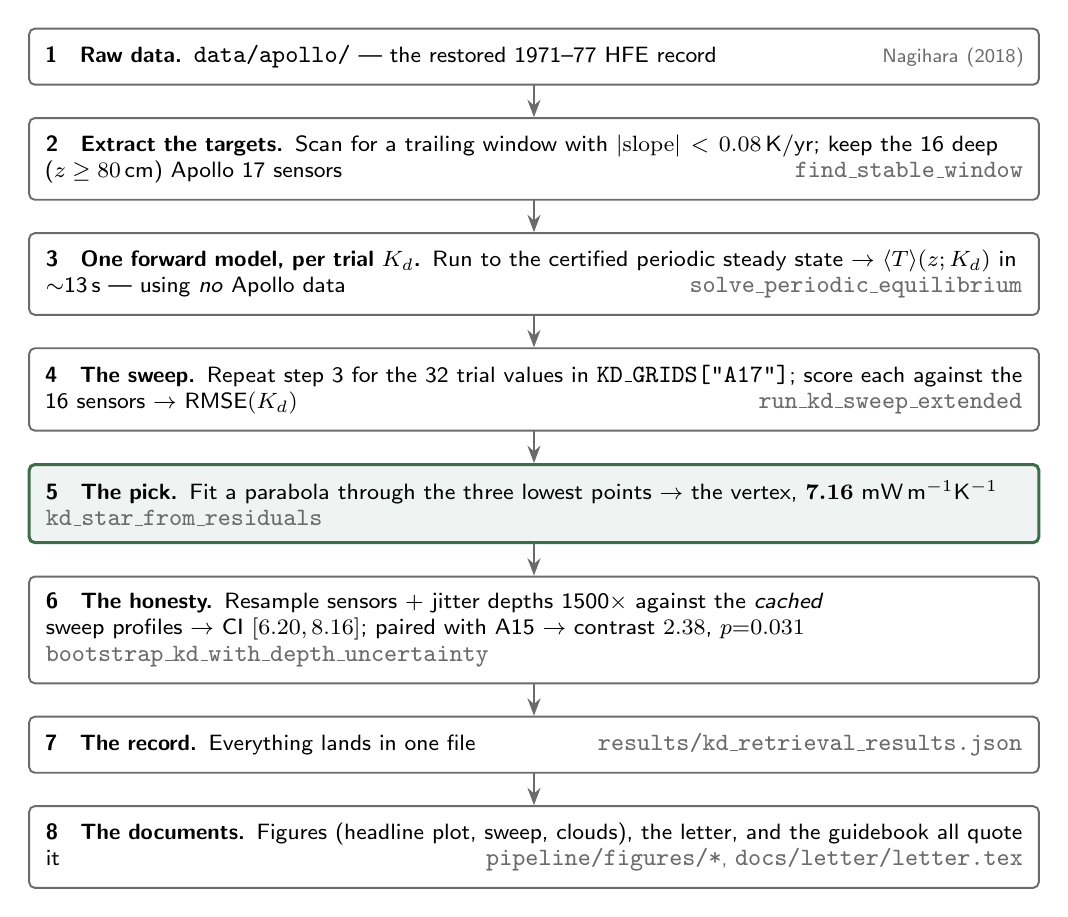
\begin{tikzpicture}[
  font=\sffamily\footnotesize,
  every node/.style={align=left},
  box/.style={rectangle, rounded corners=2pt, draw=dim, line width=0.7pt,
              fill=white, inner sep=6pt, text width=12.4cm},
  hl/.style={box, draw=forest, line width=1.1pt, fill=forest!8},
  arr/.style={-{Stealth[length=2.2mm]}, line width=0.9pt, draw=dim,
              rounded corners=2pt, line cap=round}
]
  \node[box] (s1) at (0,0)
    {\textbf{1 \; Raw data.} \code{data/apollo/} --- the restored 1971--77 HFE record \hfill {\scriptsize\color{dim}Nagihara (2018)}};
  \node[box, below=4mm of s1] (s2)
    {\textbf{2 \; Extract the targets.} Scan for a trailing window with $|{\rm slope}|<0.08$\,K/yr; keep the 16 deep ($z\geq80$\,cm) Apollo~17 sensors \hfill {\scriptsize\color{dim}\code{find\_stable\_window}}};
  \node[box, below=4mm of s2] (s3)
    {\textbf{3 \; One forward model, per trial $K_d$.} Run to the certified periodic steady state $\rightarrow$ $\langle T\rangle(z;K_d)$ in $\sim$13\,s --- using \emph{no} Apollo data \hfill {\scriptsize\color{dim}\code{solve\_periodic\_equilibrium}}};
  \node[box, below=4mm of s3] (s4)
    {\textbf{4 \; The sweep.} Repeat step~3 for the 32 trial values in \code{KD\_GRIDS["A17"]}; score each against the 16 sensors $\rightarrow$ RMSE$(K_d)$ \hfill {\scriptsize\color{dim}\code{run\_kd\_sweep\_extended}}};
  \node[hl, below=4mm of s4] (s5)
    {\textbf{5 \; The pick.} Fit a parabola through the three lowest points $\rightarrow$ the vertex, $\boldsymbol{7.16}$ mW\,m$^{-1}$K$^{-1}$ \hfill {\scriptsize\color{dim}\code{kd\_star\_from\_residuals}}};
  \node[box, below=4mm of s5] (s6)
    {\textbf{6 \; The honesty.} Resample sensors + jitter depths 1500$\times$ against the \emph{cached} sweep profiles $\rightarrow$ CI $[6.20,8.16]$; paired with A15 $\rightarrow$ contrast $2.38$, $p{=}0.031$ \hfill {\scriptsize\color{dim}\code{bootstrap\_kd\_with\_depth\_uncertainty}}};
  \node[box, below=4mm of s6] (s7)
    {\textbf{7 \; The record.} Everything lands in one file \hfill {\scriptsize\color{dim}\code{results/kd\_retrieval\_results.json}}};
  \node[box, below=4mm of s7] (s8)
    {\textbf{8 \; The documents.} Figures (headline plot, sweep, clouds), the letter, and the guidebook all quote it \hfill {\scriptsize\color{dim}\code{pipeline/figures/*}, \code{docs/letter/letter.tex}}};

  \draw[arr] (s1.south) -- (s2.north);
  \draw[arr] (s2.south) -- (s3.north);
  \draw[arr] (s3.south) -- (s4.north);
  \draw[arr] (s4.south) -- (s5.north);
  \draw[arr] (s5.south) -- (s6.north);
  \draw[arr] (s6.south) -- (s7.north);
  \draw[arr] (s7.south) -- (s8.north);
\end{tikzpicture}
\caption{Every step names the real file and function --- trace it yourself
with \code{grep} if in doubt. Change anything upstream (a constant, the grid,
$n_{\rm inner}$) and the number is only allowed to change by re-running this
chain, never by editing a document.}
\label{fig:trace}
\end{figure}

% =====================================================================
\section{``How do I\ldots?'' recipes}
% =====================================================================

\begin{center}\small
\begin{tabularx}{\textwidth}{@{}X >{\ttfamily\small}l@{}}
\toprule
\textnormal{\textbf{I want to\ldots}} & \textnormal{\textbf{Do this}} \\
\midrule
run the tests & make test \\
run one converged solve in Python & see the last cells of equilibrium\_demo.ipynb \\
get $T(z)$ at a local lunar time & profile\_at\_local\_time(eq, "14:30") \\
re-run the full retrieval ($\sim$15 min) & make retrieve \\
re-run all sensitivity/robustness numbers & make aux \\
rebuild every figure & make figures \\
rebuild one figure & python pipeline/figures/make\_<name>.py \\
rebuild a TikZ diagram & cd docs/guidebook/figures-tikz \&\& ./build.sh <name> \\
recompile the documents & make paper \\
everything from scratch & make all \\
re-measure the speed-up claims & python pipeline/compute/benchmark\_speedup.py \\
\bottomrule
\end{tabularx}
\end{center}

\noindent\textbf{Changing a physical constant:} \emph{only} in
\code{src/lunar/config.py} / \code{constants.py}, with a source comment ---
then re-run the chain and record the before/after.

% =====================================================================
\section{House rules (learned the hard way)}
% =====================================================================

These exist because each was once violated and cost real time --- the full
stories are in guidebook Ch.~5, ``Where every input comes from.''

\begin{housebox}
\begin{enumerate}[leftmargin=1.6em, itemsep=5pt]
\item \textbf{One definition per constant} (\code{config.py}). A duplicated
  $Q_b$ drifted silently and biased a headline number for weeks.
\item \textbf{A convergence criterion must test the quantity you report.}
  Cycle-to-cycle agreement passed while the deep column was 10--40\,K wrong
  (the F1 bug); $n_{\rm inner}=12$ passed its own tolerance while biasing
  $K_d^{*}$ by 0.4\,mW.
\item \textbf{Every measured claim needs a writer script.} The timing archive
  went stale the moment its one-off benchmark script was deleted;
  \code{benchmark\_speedup.py} now exists so ``measured on this machine'' is
  always re-runnable.
\item \textbf{Figures never hardcode results.} They read \code{results/*.json}
  or compute via \code{lunar} --- hardcoded values are how a headline figure
  once showed a $K_d^{*}$ three revisions old.
\item \textbf{Text on data is a build error.} Figure scripts call
  \code{assert\_no\_overlap(ax)} before saving; the build fails rather than
  shipping an overlapping label.
\end{enumerate}
\end{housebox}

\end{document}
